
\begin{abstract}
    En este documento formularemos el problema de \emph{Selective Harmonic Elimination pulse-width modulation}(SHE-PWM) como el problema de control óptimo, con el fin de encontrar soluciones de ondas cuadradas sin prefijar el número de ángulos de conmunatación. Esta nueva perspectiva nos permite realizar un análisis sobre la continuidad de soluciones.
\end{abstract}
%\tableofcontents

\section{Introduction} 

El problema \emph{Selective Harmonic Elimination}(SHE) \cite{Hoft1974} es un método de modulación que permite generar señales escalón con un espectro harmónico deseado. 
%
Es decir, dados algunos coeficientes de Fourier, el problema SHE busca la forma de onda escalón $\{f(\tau) | \tau \in (0,2\pi] \}$ cuyos coeficientes de Fourier sean los requeridos. 
%
En este contexto si el número cambios de la función es fijado el problema \emph{SHE} se puede formular como un problema de optimización donde las variables a optimizar son las localizaciones de conmutación y donde la función de coste es la distancia euclidea entre coeficientes de la función buscada y los coeficientes deseados. 

%%%%%%%%%%%%%%%%%%%%%%%%%%%%
%
Aunque el problema \emph{SHE} es fácilmente resoluble dado la configuración objetivo, el problema surge en su aplicación en tiempo real, donde la frecuencia de respuesta se encuentran en el orden de los $GHz$. 
%
No es posible calcular los ángulos de conmutación mediante una optimización a tiempo real es por ello que se precalculan las soluciones para distintos objetivos, con el fin de utilizar los resultados guardados.
%
Cuando una solución no precalculada es requerida se realizan extrapolaciones con ayuda de las demás soluciones para obtenerla. 
%
Sin embargo es conocido que el espacio de soluciones en los ángulos de conmutación es discontinuo, como se muestra en distintos estudios.

%%%%%%%%%%%%%%%%%%%%%%%%%%%%%%%%%%%%%%%%%%%%%%%%%%%%%%%%%%%

%
La naturaleza sobre la aparición y el desvanecimineto de las soluciones es desconocida. Por medio del cálculo \emph{offline} de las soluciones se sabe que mientras más ángulos de conmutación es considerado más grande es la región continua de soluciones.
%
Esto nos indíca que el número de ángulos de conmutación necesarios a lo largo de una región del espacio de soluciones podría cambiar de manera que esta formulación es poco flexible para una descripción continua de las soluciones.

%%%%%%%%%%%%%%%%%%%%%%%%%%%%%%%%%%%%%%%%%%%%%%%%%%%%%%%%%%%

%
En este documento presentaremos el problema SHE como un problema de control óptimo, donde la variable de optimización es la señal $f(\tau)$ definida en todo el intervalo $[0,2\pi]$.
%
Asi pues describiremos como en el problema SHE los coeficientes de Fourier de la función $f(\tau)$ se pueden ver como el estado final de un sistema controlado por $f(\tau)$. 
%
De manera que la optimización se realiza entre todas las posibles funciones que cumplan $|f(\tau)|<1$ que puedan controlar el estado final a los coeficientes de Fourier deseados.  Luego mostraremos como diseñar un problema de control de manera que la solución sea una función escalón. Por último, mostraremos soluciónes del problema \emph{SHE} mediante la formulación del control óptimo viendo como esta metodología es versátil ante la variación del número de conmutaciones.
%


\section{Selective Harmonic Elimination as dynamical system}

%
El problema \emph{Selective Harmonic Elimination}(SHE) consiste en la búsqueda de una función $f(\tau )$ definida en el intervalo $[0,2\pi]$, fijados unos pocos coeficientes de Fourier. Esta función $f(\tau)$ solo podrá tomar dos posibles valores $\{-1,1\}$.
%
Nos centraremos en concreto en las funciones $f(\tau)$ con simetría de media onda, es decir funciones tal que $f(\tau) = -f(\tau + \pi)$, por lo que la descripción de la función $f(\tau)$ queda determinada con sus valores en el intervalo $\tau \in [0,\pi]$. De esta forma, nos referiremos a una función $\{ f(\tau)  | \tau \in [0,\pi] \}$ cuyo desarrollo en serie de Fourier se puede escribir como:

\begin{gather}
    f(\tau ) = \sum_{i \in odd} a_i \cos(i\tau)+ \sum_{j \in odd}  b_j \sin(j \tau) 
\end{gather}

Donde $a_i$ y $b_j$  son:
\begin{gather}
    a_i = \frac{2}{\pi} \int_0^\pi f(\tau ) \cos(i \tau)d\tau \ | \ \forall i \ odd \label{an}\\
    b_j = \frac{2}{\pi} \int_0^\pi f(\tau)  \sin(j \tau) d\tau \ | \ \forall j \ odd \label{bn}
\end{gather}


Entonces el problema de SHE se puede formular como:

\begin{problem}[SHE para dos niveles]\label{SHEp}
    Dado dos conjuntos de números impares $\mathcal{E}_a$ y $\mathcal{E}_b$ con cardinalidades $|\mathcal{E}_a| = N_a$ y  $|\mathcal{E}_b| = N_b$ respectivamente, y dado los vectores objetivo $\bm{a}_T  \in \mathbb{R}^{N_a}$ y $\bm{b}_T  \in \mathbb{R}^{N_b}$, buscamos una función  $\{f(\tau ) \ | \ \tau \in (0,\pi)\}$ tal que $f(\tau)$ solo pueda tomar los valores  $\{-1,1\}$ y cuyos coeficientes de Fourier satisfagan: $ a_i = (\bm{a}_T)_i \ | \ \forall i \in \mathcal{E}_a$ y  $b_j = (\bm{b}_T)_j \ \forall \ | \  j \in \mathcal{E}_b$. 
\end{problem}





Inspirados en la naturaleza continua de la variable de optimización $f(\tau)$ proponemos en este documento la formulación desde el control óptimo. Es decir en lugar buscar los ángulos de conmutación, buscaremos la función $f(\tau) \in \{ g(\tau)  \in L^\infty([0,\pi])\ /\ |g(\tau)| < 1\} $ que tenga los coeficientes de Fourier deseados. 
%
Utilizaremos el  teorema fundamental del cálculo diferencial para re-escribir la expresión de los coeficientes de Fourier (\ref{an}) y (\ref{bn}) como la evolución de un sistema dinámico. Es decir:

\begin{gather}
    \alpha_i(\tau) = \frac{2}{\pi}\int_0^\tau f(\tau) \cos(i\tau)d\tau 
    \Rightarrow
    \begin{cases} \label{ode}
        \dot{\alpha_i}(\tau) & = \frac{2}{\pi}f(\tau)\cos(i\tau) \\  
        \alpha_i(0) & = 0       
    \end{cases}
\end{gather}

\begin{gather}
    \beta_j(\tau) = \frac{2}{\pi}\int_0^\tau f(\tau) \sin(j\tau)d\tau 
    \Rightarrow
    \begin{cases} \label{ode}
        \dot{\beta}_j(\tau) & = \frac{2}{\pi}f(\tau)\sin(j\tau) \\  
        \beta_j(0) & = 0       
    \end{cases}
\end{gather}

La evolución de los sistemas dinámicos $\alpha_i(\tau)$ y $\beta_j(\tau)$ desde el tiempo $\tau=0$ hasta $\tau=\pi$ nos da lugar a los coeficientes $a_i$ y $b_j$. 
De esta manera, el problema general de SHE (\ref{SHEp}) puede formularse como un problema de control de un sistema dinámico donde $\alpha_i(\tau) \ | \ \forall i \in \mathcal{E}_a  $ y $ \beta_j(\tau) \ \forall j \in \mathcal{E}_b$ son los estados del sistema y donde $f(\tau)$ es la variable de control, y cuyo objetivo será llevar los estados desde el origen de coordenadas hasta los vectores objetivos $\bm{a}_T$ y $\bm{b}_T$ en tiempo $\tau = \pi$ (véase figura (\ref{syscon})).



\begin{figure}
    \centering
    \begin{subfigure}[b]{0.475\textwidth}
        \centering
        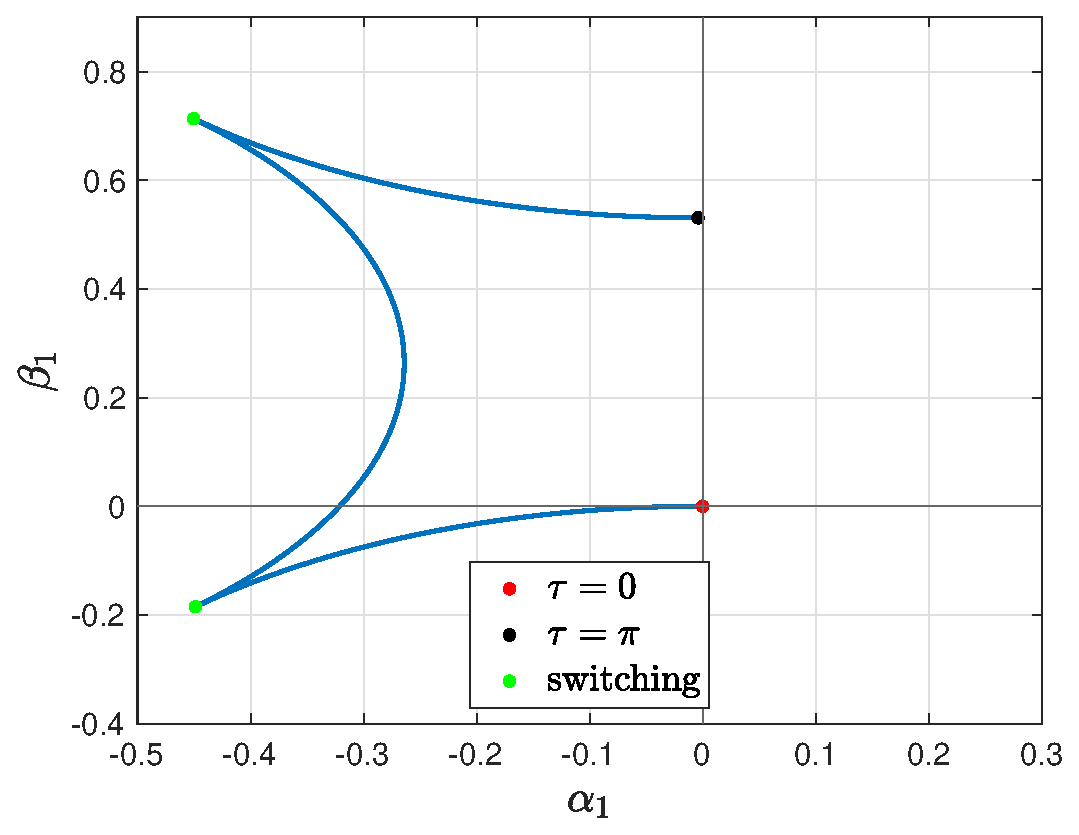
\includegraphics[width=\textwidth]{img/sys.eps}
        \caption{Dynamical System}
        \label{fig:sys}
    \end{subfigure}
    \hfill
    \begin{subfigure}[b]{0.475\textwidth}
        \centering
        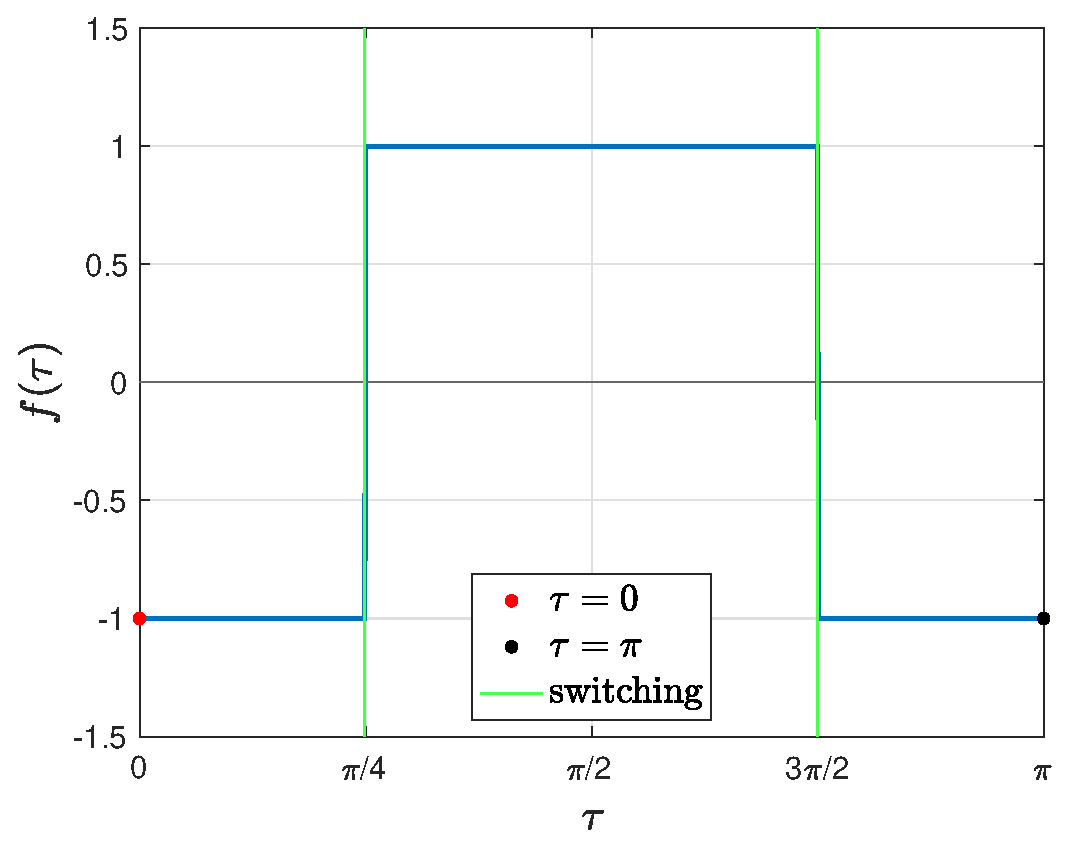
\includegraphics[width=\textwidth]{img/con.eps}
        \caption{Control}
        \label{fig:con}
    \end{subfigure}
    \caption{Mostramos el problema SHE como un sistema dinámico cuando consideramos los coeficientes de Fourier $a_1$ y $b_1$. En la figura (a) podemos ver la evolución del sistema dinámico asociado a los coeficientes de Fourier $a_1$ y $b_1$. Por otro lado, en la figura (b) podemos ver el control $f(\tau)$ que genera la trayectoria mostrada en (a).}
    \label{syscon}
\end{figure}